\documentclass[a4paper,10pt]{article}
\usepackage[utf8]{inputenc}
\usepackage{graphicx}
\usepackage[margin=1in]{geometry}
\usepackage{amsmath} %Never write a paper without using amsmath for its many new commands 
\usepackage{amssymb} %Some extra symbols 

%http://tex.stackexchange.com/questions/17489/change-caption-name-of-figures
\renewcommand{\figurename}{Step}

%http://tex.stackexchange.com/questions/58752/how-do-i-generate-a-check-list#answer-58756
\newenvironment{checklist}{%
  \small
  \begin{list}{}{}% whatever you want the list to be
  
  %http://stackoverflow.com/questions/3275622/latex-remove-spaces-between-items-in-list#3275668
  \setlength{\itemsep}{1pt}
  \setlength{\parskip}{0pt}
  \setlength{\parsep}{0pt}
  
  \let\olditem\item
  \renewcommand\item{{\olditem $\Box$} }
}{%
  \end{list}
}   

%opening
\title{Mash Cleaning}
\author{Ryan Duve}

\begin{document}

\maketitle

\begin{abstract}
\vspace{.1cm}
\fbox{\parbox{.75\textwidth}{Only workers highly familiar with the technical aspects of Hifrost are authorized to perform this procedure.
}}
\vspace{.1cm}

We suspect the dilution cooldown (10/9/2014) resulted in 10 L air getting stuck in the recovered mash in T1.  This procedure serves as a technical document to capture the air in a LN2 trap and measure the captured air in the tank T3.

\end{abstract}

\section{Prep}
\begin{figure}[htbp!]
 \centering
 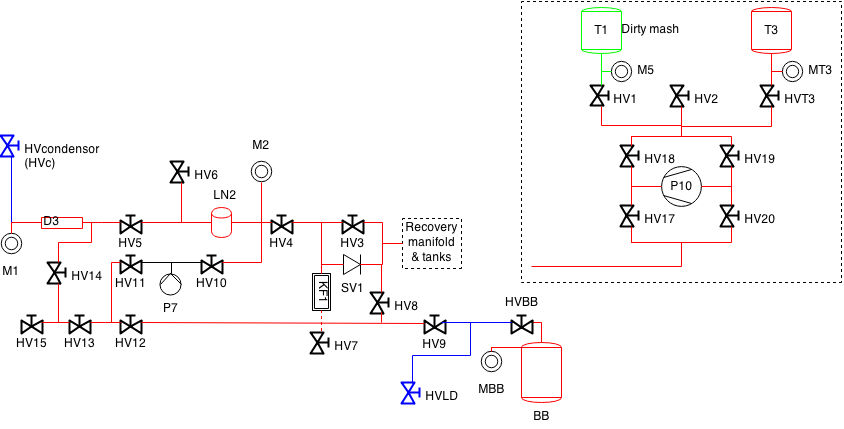
\includegraphics[width=\textwidth]{./mash-cleaning-01.png}
 % he-3-transfer-04-evac-system-with-p7.png: 0x0 pixel, 0dpi, 0.00x0.00 cm, bb=
 \caption{Red and blue volumes need to be evacuated ahead of time, blue connections are new and must be leak checked via HVLD (``hand valve - leak detector'').}
 \label{a}
\end{figure}

\begin{checklist}
 \item Regenerate LN$_2$ trap.
 \item Configure the system as shown in Step \ref{a}. Purge all lines along the red/blue paths with P7 to clean the system.
 \item Leak check the blue volumes.
 \item Close all valves; kill P7; fill trap with LN$_2$.
\end{checklist}
\pagebreak
\section{Cleaning}

\begin{figure}[htbp!]
 \centering
 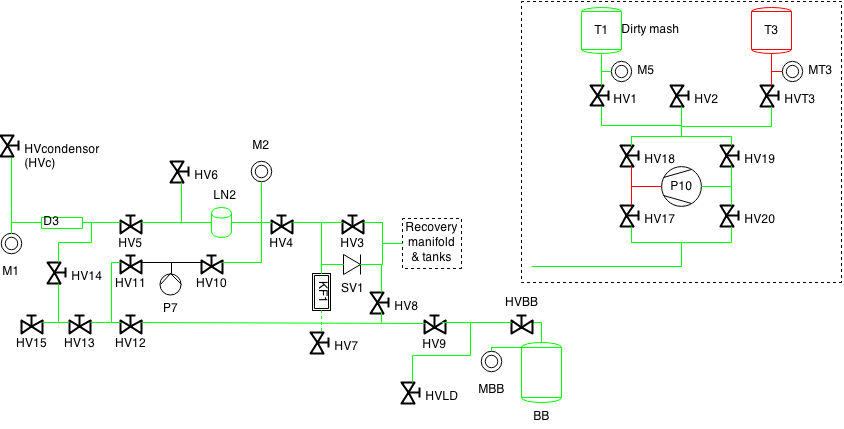
\includegraphics[width=\textwidth]{./mash-cleaning-02.png}
 % he-3-transfer-04-evac-system-with-p7.png: 0x0 pixel, 0dpi, 0.00x0.00 cm, bb=
 \caption{Open valves in this order: HV1, HV19, HV20, HV3, HV4, HV5, HV14, HV13, HV12, HV9, HVBB.  Wait until Big Blue equilibrates with T3.  The green volumes should all be at the same pressure.}
 \label{b}
\end{figure}

\begin{figure}[htbp!]
 \centering
 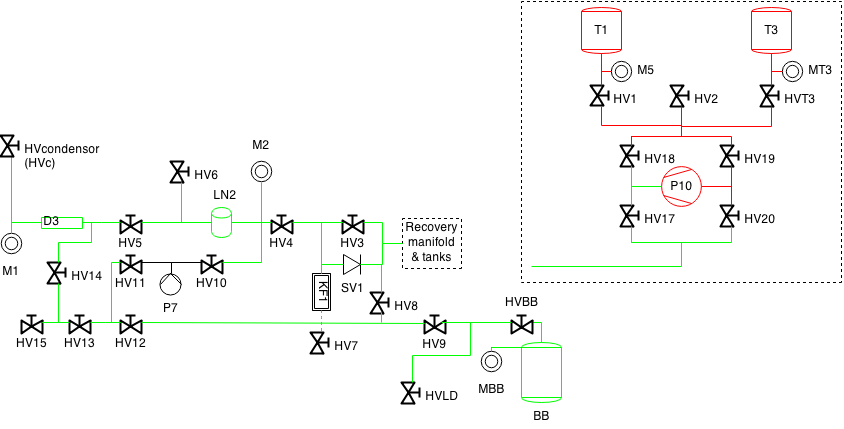
\includegraphics[width=\textwidth]{./mash-cleaning-03.png}
 % he-3-transfer-04-evac-system-with-p7.png: 0x0 pixel, 0dpi, 0.00x0.00 cm, bb=
 \caption{Close HV19, HV20; then open HV17 and turn on P10.  Slowly open HV19 and let M5 drop.}
 \label{c}
\end{figure}


\begin{figure}[htbp!]
 \centering
 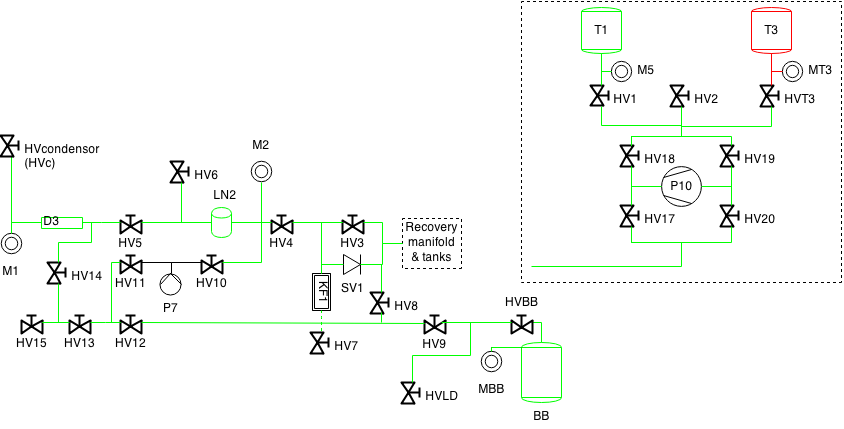
\includegraphics[width=\textwidth]{./mash-cleaning-04.png}
 % he-3-transfer-04-evac-system-with-p7.png: 0x0 pixel, 0dpi, 0.00x0.00 cm, bb=
 \caption{When M5 is around 0 mbar, close HV19, then kill P10.  Close HV17.  Open HV20 and HV19.  Wait until M5 and MBB equilibrate.}
 \label{d}
\end{figure}


\begin{figure}[htbp!]
 \centering
 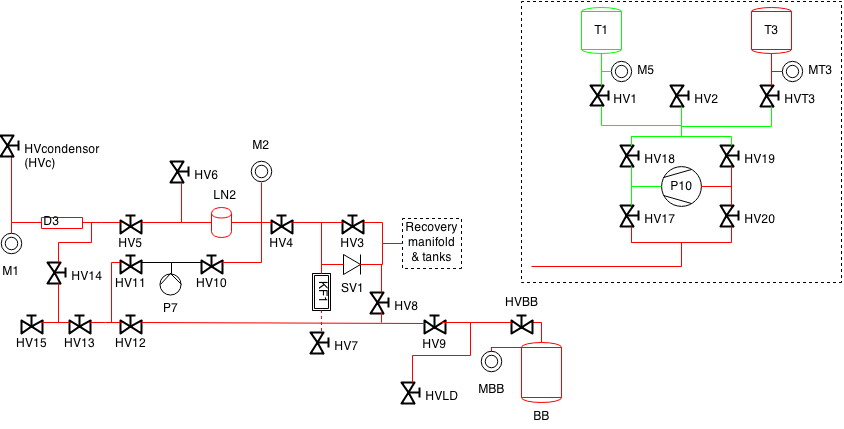
\includegraphics[width=\textwidth]{./mash-cleaning-05.png}
 % he-3-transfer-04-evac-system-with-p7.png: 0x0 pixel, 0dpi, 0.00x0.00 cm, bb=
 \caption{Close HV19 and HV20.  Open HV18 and then start P10.  Slowly open HV20; wait until MBB approaches 0.  Close HV20, kill P10, then close HV18.}
 \label{e}
\end{figure}

\begin{figure}[htbp!]
 \centering
 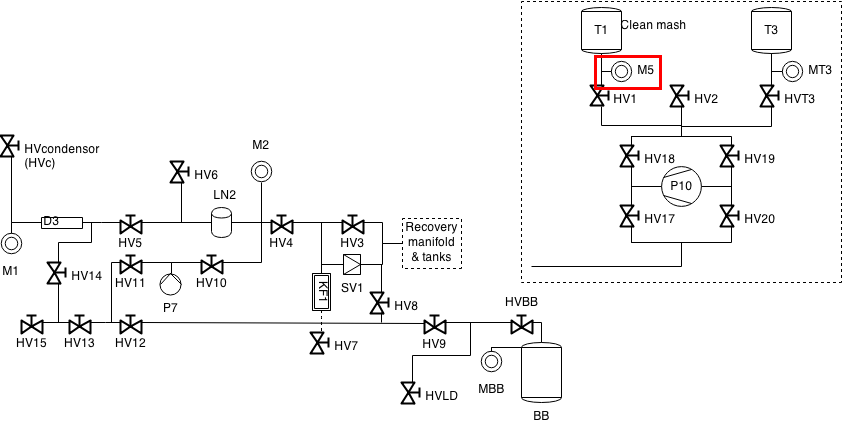
\includegraphics[width=\textwidth]{./mash-cleaning-06.png}
 % he-3-transfer-04-evac-system-with-p7.png: 0x0 pixel, 0dpi, 0.00x0.00 cm, bb=
 \caption{Repeat Steps 2-5 until M5 remains constant between passes.}
 \label{f}
\end{figure}


\begin{figure}[htbp!]
 \centering
 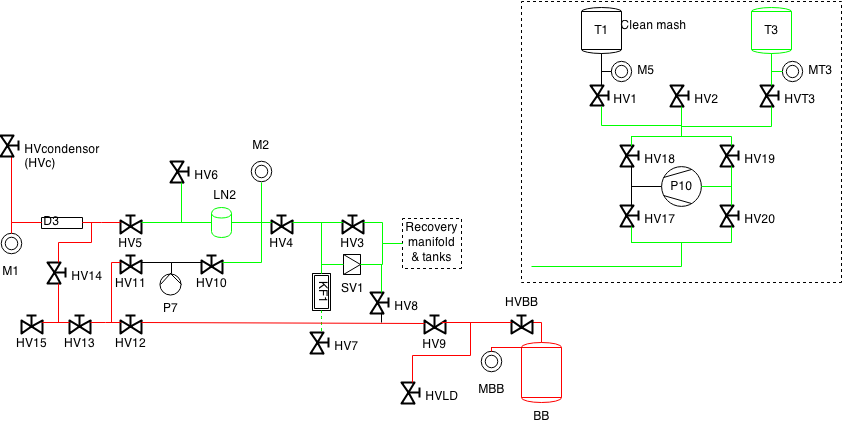
\includegraphics[width=\textwidth]{./mash-cleaning-07.png}
 % he-3-transfer-04-evac-system-with-p7.png: 0x0 pixel, 0dpi, 0.00x0.00 cm, bb=
 \caption{Close all valves, then open HV4, HV3, HV20, HV19 and HVT3.  Warm up trap and record pressure MT3 to measure how much air was removed from mash.  Use P10 to capture more air in T3 if higher precision measurement is desired.}
 \label{g}
\end{figure}


\end{document}
